\documentclass[11pt, letterpaper, includehead]{article}

%%%%%%%%%%%%%%%%%%%%% Pre-document %%%%%%%%%%%%%%%%%%%%%
\usepackage{fancyhdr}  % Allow for headers
\usepackage{graphicx}  % Allow for figures 
\usepackage{float}     % Allow for figure inserted in specified location
\usepackage{amsmath}   % Allow for aligned math
\usepackage{array}     % Allow for cell width manipulation
\usepackage{nicematrix}
\usepackage{multicol}

\setlength{\parindent}{0pt} % Remove auto paragraph indents

% Get rid of those big ass margins
\usepackage[margin=1in]{geometry}

% Table cell formatting
\setlength{\arrayrulewidth}{0.25mm}
\setlength{\tabcolsep}{11pt}
\renewcommand{\arraystretch}{1.2}

\begin{document}

%%%%%%%%%%%%%%%%%%%%% Title Page %%%%%%%%%%%%%%%%%%%%%
\begin{titlepage}
  \begin{center}
    \Huge{\textbf{Lab 5}}\\
    \Huge{Forces and Acceleration}
    \vfill
    \begin{figure}[H] % H makes the figure insert at the position in the document
      \centering 
      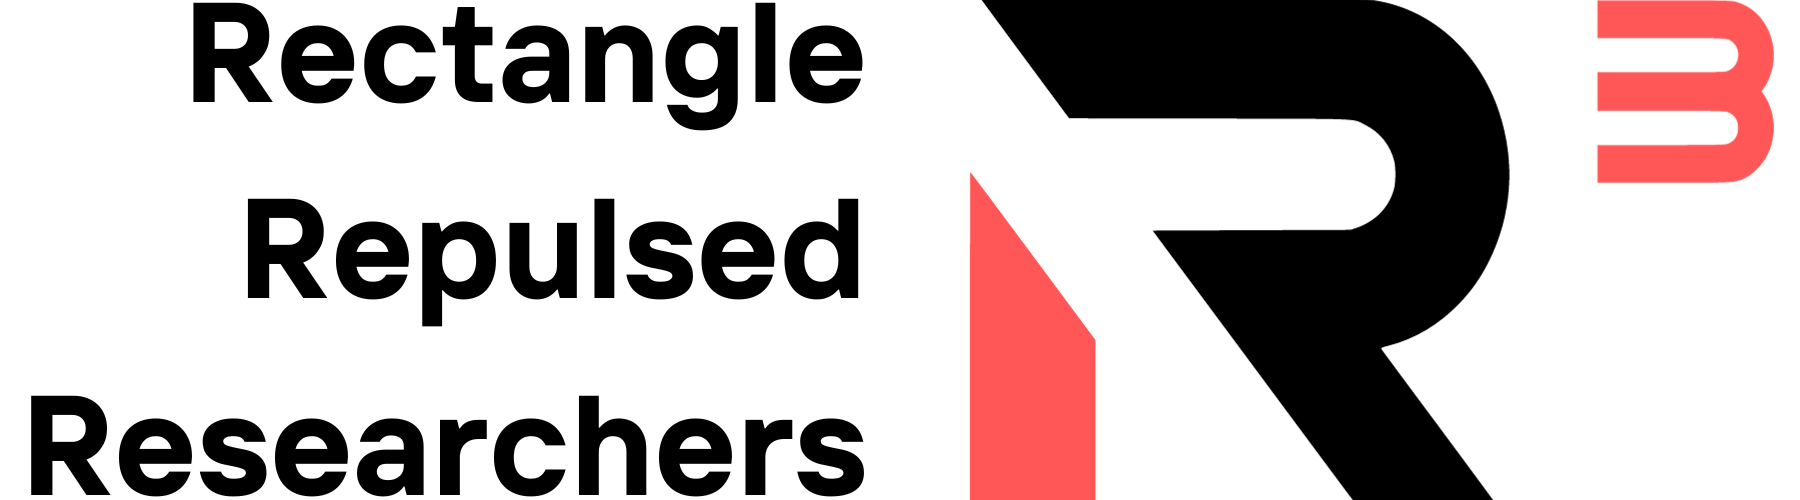
\includegraphics[width=6cm]{../logo.png}
    \end{figure}
    \large{\textbf{your name here}}\\
    \large{Julian Barossi, Liam Gilligan, Stephanie L'Heureux}\\
    \vspace{0.5cm}
    \normalsize
    \today
  \end{center}
\end{titlepage}

%%%%%%%%%%%%%%%%%%%%% TABLE OF CONTENTS %%%%%%%%%%%%%%%%%%%%%
\tableofcontents
\pagebreak % Move to next page

% Add a nice fancy header
\pagestyle{fancy}
\fancyhead{}
\fancyhead[C]{\textbf{Lab 5:} Forces and Acceleration}

\section{Level track} % 1
\subsection{Free body diagram} % 1.1
\subsection{Predicted acceleration of the system} % 1.2
\subsection{Predicted time} % 1.3
\subsection{Experimental time} % 1.4
\subsection{Analysis} % 1.5
\subsection{Tension} % 1.6
\section{Sloping air track I} % 2
\subsection{Free body diagram}
\subsection{Predicted acceleration of the system}
\subsection{Predicted time}
\subsection{Experimental time}
\subsection{Analysis}
\section{Sloping air track II} % 3
\subsection{Free body diagram}
\subsection{Predicted acceleration of the system}
\subsection{Predicted time}
\subsection{Experimental time}
\subsection{Analysis}
\subsection{Tension}

\end{document}
